\documentclass[11pt]{jreport}
\usepackage{wuse_thesis}
\usepackage{indentfirst}
\usepackage{color}
\usepackage{url}	% \url{}コマンド用.URLを表示する際に便利
\newcommand{\todo}[1]{\colorbox{yellow}{{\bf TODO}:}{\color{red} {\textbf{[#1]}}}} 	
\usepackage{graphicx}  % ←graphicx.styを用いてEPSを取り込む場合有効にする
\usepackage{tabularx}
\usepackage{multirow}
\usepackage[hang,small,bf]{caption}
\usepackage[subrefformat=parens]{subcaption}
\usepackage{here}
\usepackage{amsmath}

% 他のパッケージ・スタイルを使う場合には適宜追加	

%%%%%%%%%%%%%%%%%%%%%%%%%%%%%%%%%%%%%%%%%%%%%%%%%%%%%%%%%%%%%%%%%%%%%%%%

%%
%% 主に表紙を作成するための情報
%%

%%  タイトル(修論の場合は英語表記も指定)
\title{オブジェクトの動作に基づく\\
	Scratch作品の直感的検索手法}

%\title{オブジェクト動作経路の時系列解析に基づくビジュアルプログラム作品検索の試み}       

%\etitle{Test\\Test\\Test}

%%  著者名(修論の場合は英語表記も指定)
\author{福地 ユキ}
%\eauthor{Akinori Ihara}

%% 卒業論文・修士論文(以下のどちらかを選択)
\bachelar	% 卒業論文(4年生用)
%\master  	% 修士論文(M2用)

%%  学科・クラスタ
\department{システム工}
%\department{デザイン情報}
%\department{デザイン科学}

%%  学生番号
\studentid{60236238}

%%  卒業年度
\gyear{2021}		% 提出年が2022年なら,2021年度

%%  論文提出日
\date{2022年2月15日}	% 修士の場合は月(2021年2月)までとし,英語表記も指定
%\edate{February 2021}	% 修士の場合,こちら(英語表記)も有効化

%%%%%%%%%%%%%%%%%%%%%%%%%%%%%%%%%%%%%%%%%%%%%%%%%%%%%%%%%%%%%%%%%%%%%%%%

\begin{document}

\maketitle

%%
%%  概要
%%
\begin{abstract}

ビジュアルプログラミング言語は,視覚的に表現された命令処理を操作することで
プログラムを実装可能なプログラミング言語である.
ビジュアルプログラミング学習サービスの1つであるScratchでは,
ユーザが制作したプログラム作品をオンラインサービス上に公開可能である.
Scratchのオンラインサービス上には,多数のユーザが制作した膨大な数の作品が公開されており,
ユーザは他者の作品を参照することで多様な実装方法を学習する.
参照する他者の作品を探し出すためにキーワード検索を行うが,ユーザがイメージする動作を言語化することは難しく,
動作に関するキーワードをタイトルや説明文に含まない作品は検索不可能であるため,
ユーザがイメージする動作を含む作品を検索することは容易ではない.
キーワードによる検索ではなく,マウスを用いた描画等によって動作のイメージを入力とする
直感的な検索を実現することで,ユーザがイメージする動作を含む作品の検索を容易にできると考える.

本研究では,動作のイメージを入力とする,オブジェクトの動作に基づくScratch作品の直感的検索手法を提案する.
入力と検索対象の各動作の類似度合いを測るために,
2つの時系列データの距離を算出する動的時間伸縮法を用いる.類似動作を抽出可能な距離を明らかにするために,
13,437件の公開作品を対象に入力を行い,距離算出結果の分析を行なった.
分析では,入力との距離が異なる複数の動作を被験者に提示し,被験者全員が類似していない
と判断する値よりも近い距離を,類似動作を抽出可能な距離とした.
結果は,〜.\todo{結果を載せる}

本研究は,動作のイメージを入力とするScratch作品の直感的検索手法を提案することで
検索を容易にし,他者の作品を参照することによる実装方法の学習が促進されることを期待する.

\end{abstract}

%%  目次
\tableofcontents

%%  図目次 (図目次をいれたければ以下のコメントをはずす)
%\listoffigures

%%  表目次 (表目次をいれたければ以下のコメントをはずす)
%\listoftables

\newpage
\pagenumbering{arabic}	% 以降のページ番号を算用数字に

%%%%%%%%%%%%%%%%%%%%%%%%%%%%%%%%%%%%%%%%%%%%%%%%%%%%%%%%%%%%%%%%%%%%%%%%

%%
%%  本文はここから
%%


\chapter{はじめに}

初等教育からのプログラミング必修化に伴い,プログラミング教育が進められている.
特に,テキストの入力ではなく,視覚的に表現された命令処理の操作でプログラムを実装する
ビジュアルプログラミング言語が利用されている.
ビジュアルプログラミング言語は,直感的にプログラムを実装可能なことや,
視覚的に表現されたプログラムの理解が容易であること,
テキストベースのプログラミング言語で障壁となるテキスト入力の間違いが発生しないことなどから,
プログラミング初学者が取り組みやすい言語となっている.

ビジュアルプログラミング言語を用いた代表的な学習サービスScratch\footnote{ \url{https://scratch.mit.edu/}}は,
ユーザが制作したプログラム作品をタイトル・説明文を添えてオンラインサービス上に公開可能である.
2022年1月時点で8,300万以上の人がScratchに登録しており,
オンラインサービス上に9.400万件以上のプログラム作品を公開している
\footnote{\url{https://scratch.mit.edu/statistics/}}.
Scratchユーザは,オンラインサービス上の他者の作品を参照することで多様な実装方法を学習する\cite{spfa}.
参照する作品を探し出すために,ユーザは作品のタイトルと説明文を対象としたキーワード検索を行う.
しかしユーザにとって,イメージする動作を検索キーワードへ変換することは難しく,
動作に関するキーワードをタイトルや説明文に含んでいない作品を検索することは不可能であるため,
ユーザのイメージを含む作品の検索は容易ではない.
作品検索が容易ではないという課題は,他者の作品を参照する学習の障壁になると示唆する.
キーワードによる検索ではなく,動作のイメージを入力とするScratch作品の直感的な検索を実現することで,
ユーザがイメージする動作を含む作品の検索を容易にできると考える.

本論文では,マウスを用いた描画等によって動作のイメージを入力とし,
オブジェクトの動作に基づくScratch作品の直感的検索手法を提案する.
入力と検索対象の各動作の類似度合いを測るために,2つの時系列データの距離を算出する動的時間伸縮法を用いる.
類似動作を抽出可能な距離を明らかにするために,13,437件の公開作品を対象に入力を行い,
距離算出結果から入力と動作の類似性を評価する定性分析を行う.
動作のイメージを入力とするScratch作品の直感的検索手法を提案することで
検索を容易にし,他者の作品を参照することによる実装方法の学習の支援を期待する.

続く2章では,Scratchにおけるプログラム作品検索の背景と課題について述べる.
3章では提案手法について説明し,
4章では入力に類する動作を抽出可能な距離の分析とその結果について述べる.
5章では分析結果を考察し,最後に6章でまとめを述べる.


\chapter{ビジュアルプログラミング言語Scratchにおけるプログラム作品検索}

\section{Scratch}
Scratch\footnote{ \url{https://scratch.mit.edu/}}は,MITメディアラボが開発している
ビジュアルプログラミング言語の1つである.
Scratchは「10歩動かす」「15度回す」などの命令処理をブロックで視覚的に表現し,
複数のブロックを組み合わせることで,画面上のオブジェクトを動かすプログラム作品を制作する.
Scratchで制作される作品の種類は,ゲームやストーリー,アニメーションなど多岐に渡る\cite{wild}.
Scratchは,直感的にプログラムを実装可能なことや,視覚的に表現されたプログラムの理解が容易であること,
テキストベースのプログラミング言語で障壁となるテキスト入力の間違いによる構文エラーが発生しないことなどから,
プログラミング初学者が取り組みやすいプログラミング言語となっている.
従来研究では,Scratchを用いた学習がプログラミング学習に有効であり,テキストベースのプログラミング言語への
移行を容易にすることを明らかにしている\cite{blocktotext}\cite{blockandbeyond}.

図\ref{scratchdisplay}は,Scratch3.0における作品制作画面を示す.
作品は主に「ブロック」「スクリプト」「スプライト」の3つの要素で構成されている.

\begin{itemize}
    \item ブロック: 視覚的に表現された命令処理を1つのブロックで表現する.
    図\ref{scratchdisplay}の(1)に示す複数のブロックを繋ぎ合わせて使用する.
    命令処理の種類によって形状や色が異なる.表\ref{blockshape}は形状の種類と性質,
    表\ref{blockcolor}は色の種類と性質を示す.
    \item スクリプト: 複数のブロックを組み合わせて制作したひとまとまりのプログラムである.
    スクリプトはイベント駆動型であり,図\ref{scratchdisplay}の(2)に示すスクリプトの例では,
    スペースキーが押された際にプログラムが実行される.
    \item スプライト: キャラクター等の画像のオブジェクトである.
    図の〜に示すスクリプトエリアにブロックを配置しスクリプトを制作することで,プログラムをスプライトに実行させる.
    プログラム作品制作の初期画面では,図\ref{scratchdisplay}の(3)に示すCatがあらかじめ配置されている.
    ユーザはスプライトを複数配置することができ,Scratchで用意されているデフォルトの画像や,
    ユーザが創作した画像をスプライトとして使用可能である.
\end{itemize}

図\ref{scratchdisplay}に示す例では,スペースキーが押された際にCatのスプライトが
「こんにちは!」と発言し,その後進行方向に10歩移動する動作を10回繰り返す作品である.

Scratchで制作した作品は,図\ref{scratchdisplay}の(1)に示すタイトルと
図\ref{scratchdisplay}の(2)に示す説明文を添えてオンラインサービス上に公開することができる.
2022年1月時点で,8,300万人以上の人がScratchに登録しており,
オンラインサービス上に9.400万件以上の作品を公開している
\footnote{\url{https://scratch.mit.edu/statistics/}}.
他者の公開作品のプログラムを閲覧できるため,ユーザは他者の公開作品を参照することで
多様な実装方法を学習できる\cite{spfa}.

\begin{figure}[H]
    \centering
    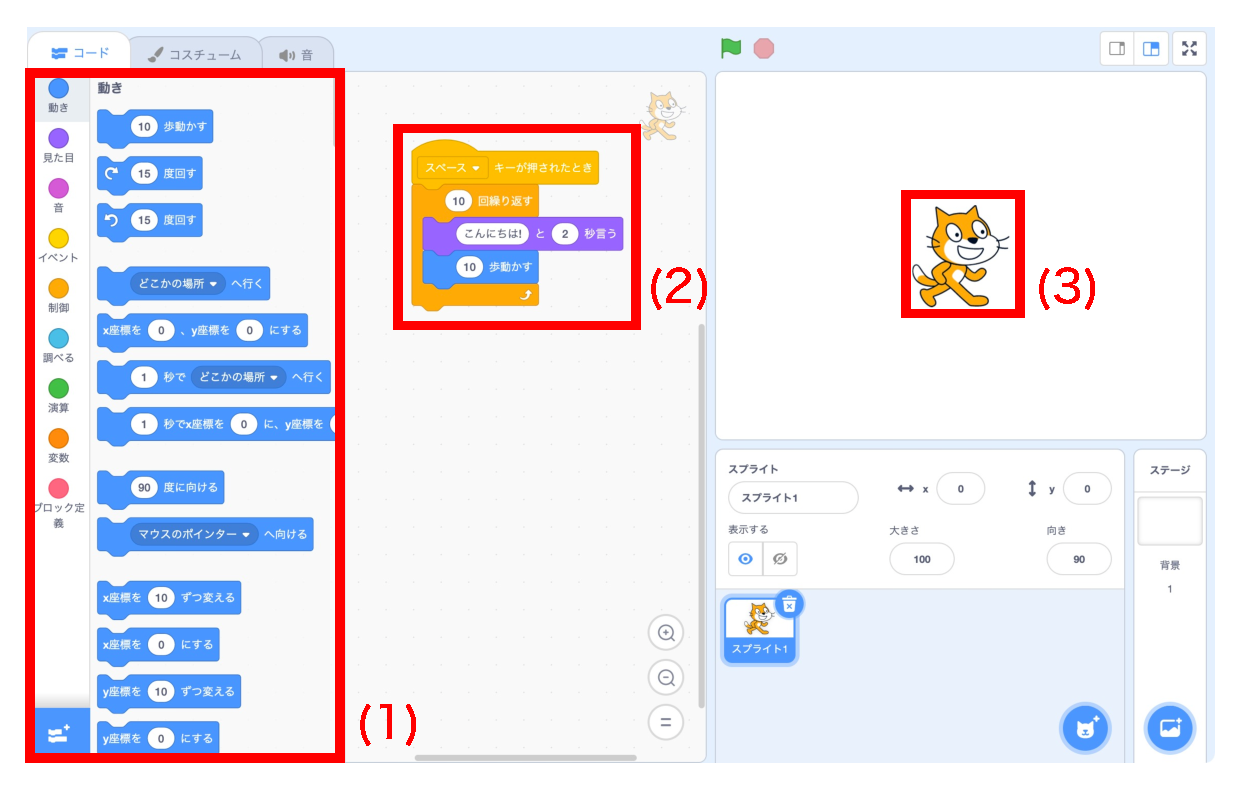
\includegraphics[width=12cm]{scratch_display.eps}
    \caption{Scratchの作品制作画面}
    \label{scratchdisplay}
\end{figure}

\begin{figure}[H]
    \centering
    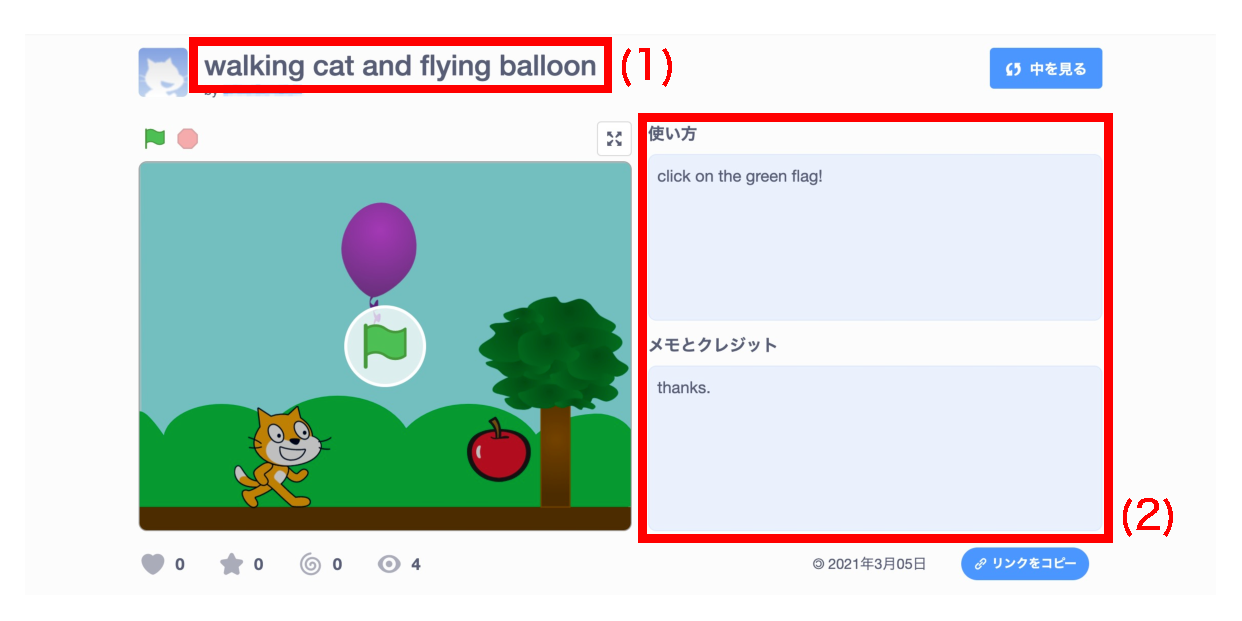
\includegraphics[width=15cm]{scratch_online.eps}
    \caption{公開したScratch作品画面}
    \label{scratchonline}
\end{figure}

\begin{table}[H]
  \caption{ブロックの形状と名前と性質}
  \label{blockshape}
  \centering
  \begin{tabularx}{\textwidth}{l|l|X}
    \hline
    \multicolumn{1}{c|}{ブロックの形状} & \multicolumn{1}{c|}{名前} & \multicolumn{1}{c}{性質} \\
    \hline \hline
    \begin{minipage}{30mm}
      \centering
      \scalebox{0.8}{
\includegraphics{press_greenflag.eps}}
    \end{minipage} & ハットブロック &  スクリプトの処理を開始するブロック \\
    \hline
    \begin{minipage}{30mm}
      \centering
      \scalebox{0.8}{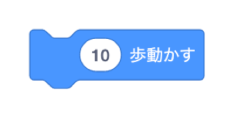
\includegraphics{walk.eps}}
    \end{minipage} & スタックブロック &  記述された命令を実行するブロック \\
    \hline
    \begin{minipage}{30mm}
      \centering
      \scalebox{0.8}{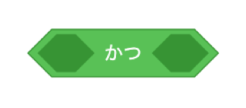
\includegraphics{and.eps}}
    \end{minipage} & 真偽ブロック &  真偽値を保持し,他のブロックの引数となるブロック \\
    \hline
    \begin{minipage}{30mm}
      \centering
      \scalebox{0.8}{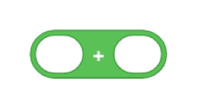
\includegraphics{add.eps}}
    \end{minipage} & 値ブロック &  値を保持し,他のブロックの引数となるブロック \\
    \hline
    \begin{minipage}{30mm}
      \centering
      \scalebox{0.8}{
\includegraphics{forever.eps}}
    \end{minipage} & C型ブロック &  間にあるブロックに対して,条件分岐や繰り返しを実行するブロック \\
    \hline
     \begin{minipage}{30mm}
      \centering
      \scalebox{0.8}{
\includegraphics{stop.eps}}
    \end{minipage} & キャップブロック &  スクリプトの処理を停止するブロック \\
    \hline
  \end{tabularx}
\end{table}

\begin{table}[H]
  \caption{ブロックの色と名前と性質}
  \label{blockcolor}
  \centering
  \begin{tabularx}{\textwidth}{l|l|X}
    \hline
    \multicolumn{1}{c|}{ブロックの色} & \multicolumn{1}{c|}{名前} & \multicolumn{1}{c}{性質} \\
    \hline \hline
    \begin{minipage}{30mm}
      \centering
      \scalebox{0.8}{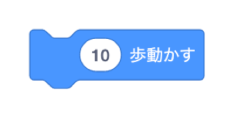
\includegraphics{walk.eps}}
    \end{minipage} & 動きブロック & スプライトを動かすブロック \\
    \hline
    \begin{minipage}{30mm}
      \centering
      \scalebox{0.8}{
\includegraphics{size.eps}}
    \end{minipage} & 見た目ブロック &  スプライトの見た目を制御するブロック \\
    \hline
    \begin{minipage}{30mm}
      \centering
      \scalebox{0.8}{
\includegraphics{sound.eps}}
    \end{minipage} & 音ブロック &  BGMやSEをいった音を制御するブロック \\
    \hline
    \begin{minipage}{30mm}
      \centering
      \scalebox{0.8}{
\includegraphics{press_greenflag.eps}}
    \end{minipage} & イベントブロック &  スクリプト実行のトリガーとなるブロック \\
    \hline
    \begin{minipage}{30mm}
      \centering
      \scalebox{0.8}{
\includegraphics{forever.eps}}
    \end{minipage} & 制御ブロック &  スクリプトを制御するブロック \\
    \hline
     \begin{minipage}{30mm}
      \centering
      \scalebox{0.8}{
\includegraphics{press_mouse.eps}}
    \end{minipage} & 調べるブロック &  スプライトや操作などの状態を調べるブロック \\
    \hline
    \begin{minipage}{30mm}
      \centering
      \scalebox{0.8}{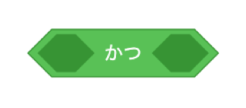
\includegraphics{and.eps}}
    \end{minipage} & 演算ブロック &  数値や論理,文字列に対する演算を行うブロック \\
    \hline
    \begin{minipage}{30mm}
      \centering
      \scalebox{0.8}{
\includegraphics{variable.eps}}
    \end{minipage} & 変数ブロック &  変数とリストを扱うブロック \\
    \hline
    \begin{minipage}{30mm}
      \centering
      \scalebox{0.8}{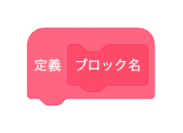
\includegraphics{define.eps}}
    \end{minipage} & ブロック定義ブロック &  メソッドを定義するブロック \\
    \hline
  \end{tabularx}
\end{table}

\section{Scratch作品の検索}

ユーザは,Scratchオンラインサービス上に公開されている膨大な数の
プログラム作品を参照することで多様な実装方法を学習することができる\cite{spfa}.
参照する作品を探し出すために,ユーザは作品のタイトルと説明文を対象としたキーワード検索を行う.
C言語やJavaをはじめとするテキストベースのプログラミング言語では
メソッド名などのキーワードを使ったプログラム検索の研究が多数行われている\cite{codesearch}.
しかし,Scratch作品の検索において,ユーザがイメージする動作を検索キーワードへ変換することは難しく,
動作に関するキーワードをタイトルや説明文に含んでいない作品を検索することは不可能であるため,
ユーザのイメージする動作を含む作品の検索は容易ではない\cite{behavior}.
キーワードではなくマウスを用いた動作描画等の直感的な操作による検索を可能にすることで,
ユーザのイメージする動作を入力とする検索が可能となり,作品検索が容易になると考える.

本論文では,動作のイメージを入力とするScratch作品の直感的検索システム実現に向けて,
類似動作を抽出する手法を提案する.
図\ref{searchsystem}は,本論文で提案する手法を用いることで
実現を期待するScratch作品の直感的検索システムの概略図を示す.
続く第3章では,提案手法について述べる.

\begin{figure}[H]
    \centering
    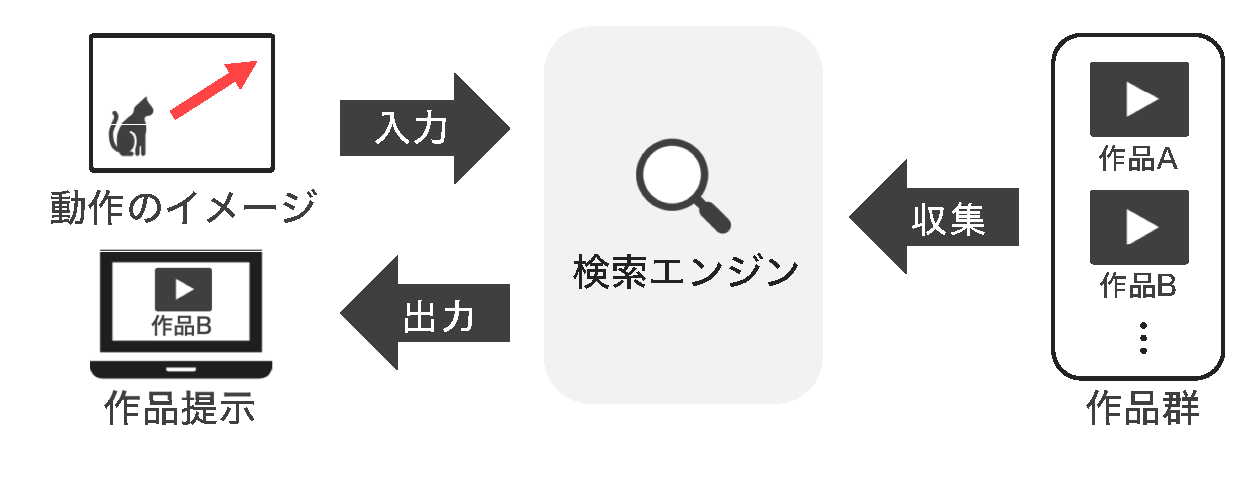
\includegraphics[width=15cm]{system.eps}
    \caption{Scratch作品の直感的検索システムの概略図}
    \label{searchsystem}
\end{figure}


\chapter{Scratch作品に含まれる類似動作の抽出手法}

\section{概要}
本章では,動作のイメージを入力とするScratch作品の直感的検索手法を述べる.
図\ref{flow}は,手法の概略図を示す.
手順1では,入力となる動作のイメージの座標の時系列データをマウスによる描画で取得し,
検索対象のScratch作品に含まれるオブジェクトの座標の時系列データを画像認識を用いて取得する.
手順2では,手順1で取得した入力と各動作の時系列データ同士の距離を算出する.
算出結果のうち,距離が近い動作を入力と類する動作として抽出する.
類似動作を抽出する距離については,4章で分析及びその結果について述べ,5章で考察について述べる.

\begin{figure}[H]
    \centering
    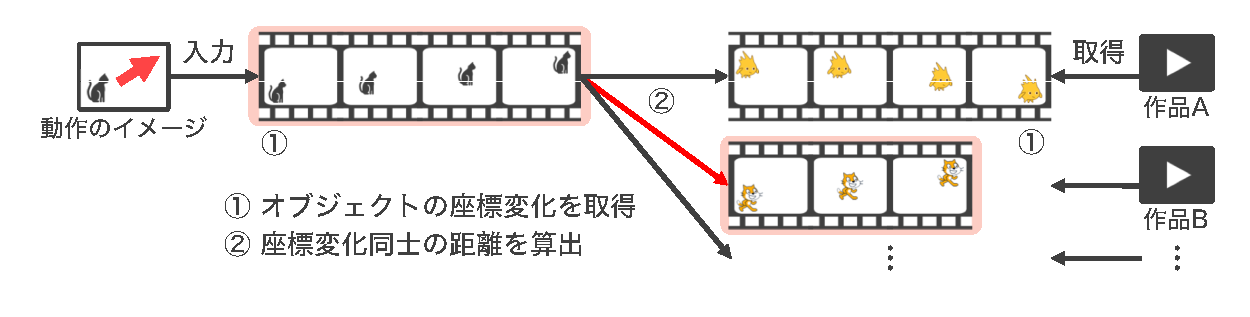
\includegraphics[width=15cm]{flow.eps}
    \caption{動作のイメージに基づく検索手法の概略図}
    \label{flow}
\end{figure}

\section{オブジェクトの座標の時系列データ取得}

\subsection{動作イメージの入力}
ユーザの持つ動作のイメージを,マウスで描画することによって入力する.
動作のイメージを描画中,軌跡を十分再現可能である0.2秒ごとにマウスの座標を取得する.
取得した座標を,入力の座標変化の時系列データとする.

\subsection{検索対象作品に含まれるオブジェクトの動作}
\label{objectbehavior}
\subsubsection{検索対象作品の収集}
Webアプリケーションの自動テストツールSelenium\footnote{https://www.selenium.dev/}を用いて,
Scratchのオンラインサービス上に公開されている作品のスナップショットを収集する.
スナップショットは,入力と同様の間隔で時系列データを取得するため0.2秒に1枚を収集する.
作品の中には実行が終わらない作品も存在するため,
該当する作品に対しては,最大100枚のスナップショットを収集する.
また,スナップショット収集を自動化するため,キー入力やマウス操作を必要としない作品を対象とする.

\subsubsection{画像認識による時系列データ取得}
収集した各作品のスナップショット中に存在する,テンプレート画像と同じ画像を用いたオブジェクトの座標を,
Loweが提案したSIFT(Scale-Invariant Feature Transform)\cite{sift}を用いた画像認識を行うことで座標変化を取得する.
SIFTは,画像中の特徴点検出と特徴量記述を行うアルゴリズムであり,照明変化や回転・拡大縮小に頑健である.
Scratchでは,オブジェクトとなるスプライトの色の変更や回転・拡大縮小を自由にできることから,
そのような変更を行なった作品にも対応するため,照明変化や回転・拡大縮小に頑健であるSIFTを採用する.
SIFTによる画像認識の手順は,以下の通りである.
\begin{enumerate}
     \item \textgt{スケール空間における極値検出:} 拡大縮小による不変性を得るため,対象とする点の特徴をより表現可能な
    近傍領域の範囲を決定する.近傍領域の範囲を決めるパラメータをスケールという.
    スケール$s$の異なるガウス関数$G(x,y,s)$と入力画像$I(x,y)$を畳み込んだ平滑化画像$L(x,y,s)$を以下の式により作成する.
    \begin{eqnarray}
        L(x,y,s) = G(x,y,s) * I(x,y) \\
        G(x,y,s) = \frac{1}{2\pi s^2} \exp (- \frac{x^2+y^2}{2s^2})
    \end{eqnarray}
    特徴点候補はスケールの異なる平滑化画像間の差分を取るDoG(Difference of Gaussian)画像$D(x,y,s)$から決定する.
    D(x,y,s)は以下の式から求める.
    \begin{eqnarray}
        D(x,y,s) = L(x,y,s_{i+1}) - L(x,y,s_i)
    \end{eqnarray}
    この処理を複数の異なるスケール間で行うことで複数のDoG画像を取得し,得られたDoG画像から極値を検出する.
    極値の検出はDoG画像を3枚1組にして行う.極値を検出するDoG画像中のある画素に注目し,その周りの26近傍を比較する.
    注目画素が極値であった場合,その画素を特徴点候補として検出する.
    \item \textgt{特徴点のローカライズ:} 特徴点候補の中にはエッジ上の点が含まれており,ノイズの影響を受けやすい.
    そのため,エッジ上に存在する特徴点候補を削除することで安定した特徴点を絞り込む.
    エッジ上の特徴点候補を削除するために,各候補における二次元ヘッセ行列を以下の式から求める.
    \begin{eqnarray}
        H = \begin{bmatrix}
            D_{xx} & D_{xy} \\
            D_{xy} & D_{yy}
        \end{bmatrix}
    \end{eqnarray}
    Hから求められる第1固有値を$\alpha$,第2固有値を$\beta$とし,その比率を$\gamma$とすると以下の式が成り立つ.
    \begin{eqnarray}
        \alpha = \gamma\beta
    \end{eqnarray}
    よって,
    \begin{eqnarray}
        \frac{Tr(H)^2}{Det(H)} = \frac{(\alpha + \beta)^2}{\alpha\beta} = \frac{(\gamma + 1)^2}{\gamma}
    \end{eqnarray}
    となり,この値を閾値処理することで不要な特徴点の除去を行う.
    \item \textgt{回転角の計算:} 検出した各特徴点に対して,回転角を割り当てる.特徴点が検出された平滑化画像の
    各画素の勾配$m(x,y)$とその勾配方向$\theta(x,y)$を以下の式から求める.
    \begin{eqnarray}
        m(x,y) = \sqrt{f_x(x,y)^2 + f_y(x,y)^2} \\ 
        \theta(x,y) = \tan^{-1}\frac{f_y(x,y)}{f_x(x,y)}
    \end{eqnarray}
    \begin{eqnarray}
        \begin{cases}
            {f_x(x,y) = L(x+1,y) - L(x-1,y)} \\
            {f_y(x,y) = L(x,y+1) - L(x,y-1)} \\
        \end{cases}
    \end{eqnarray}
    求めた勾配$m$の大きさと勾配方向$\theta$から,重み付き方向ヒストグラムを作成する.
    作成したヒストグラムから最大値となる方向を特徴点の回転角として割り当てる.
    \item \textgt{特徴量の算出:} 特徴点の周辺領域を,3で割り当てた方向を基準とした軸に回転させる.
    この状態で特徴量を算出するため,回転に対する不変性を得ることができる.
    特徴点に対して周囲の$16×16$画素を取り出し,この領域を16個の$4×4$の小領域に分割する.
    各小領域に対してビンの数が8となるヒストグラムを作成する.
    結果として$8×16=128$個の特徴量が算出される.
    \item \textgt{特徴点のマッチング: } 2枚の画像間の特徴点のマッチングを,
    最も距離の近い点を探す最近傍探索によって行う.
\end{enumerate}

本研究では,インテルが開発・公開しているオープンソースライブラリのOpenCV\footnote{https://opencv.org/}
を利用し,SIFTを用いた画像認識を行う.

Scratchでは,ユーザが自由にオブジェクトの画像を作成することができ,
オンラインサービス上に公開されている作品で使用されているオブジェクト画像が多種多様であることから,
全てのオブジェクトを対象とするのではなく,
Scratchにおいてデフォルトで用意されているオブジェクト画像339件のみを画像認識のテンプレート画像とする.

本提案手法では,動作するオブジェクトを捉えるため,
オブジェクトの動作を命令する動きブロックを使用している作品を対象とする.
1作品には複数の動作を含んでいるため,連続したスナップショット中で,
オブジェクトが登場しないフレームまでを1つの動作とする.
1動作ごとに取得した座標を,検索対象動作の座標の時系列データとする.

\section{座標の時系列データの距離算出}

\subsection{時系列データの正規化}
入力と抽出対象動作の座標が離れていても,動作の軌跡が類似していれば類似動作として抽出を行うため,
手順1で取得した時系列データを最小値0,最大値1に正規化する.

\subsection{DTW距離の算出}
入力の時系列データと,各動作の時系列データの距離を,
動的時間伸縮法(DTW: Dynamic time warping)を用いて算出する.
DTWは,2つの時系列データの距離を動的計画法に基づいて算出する手法である.
DTWでは2つの時系列データの各点の距離を総当たりで算出し,
全て求めた上で2つの時系列データの累積距離が最短となる経路を探し,
最短経路における累積距離が2つの時系列データの距離を示す.
異なる長さの時系列データ同士でも距離を算出可能である.
図\ref{dtw}に示すように,距離を算出する2つの時系列データ$S=s1,s2,...s15,T=t1,t2,...,t10$
を横と縦に並べ,点(i,j)における要素siとtj間の距離を算出する.
図中では,要素のマスの色が薄いほど距離が近く,濃いほど距離が遠いことを示す.
時系列データSとTの各要素の累積距離が最も短くなる経路を探すことで距離を算出する.

\begin{figure}[H]
    \centering
    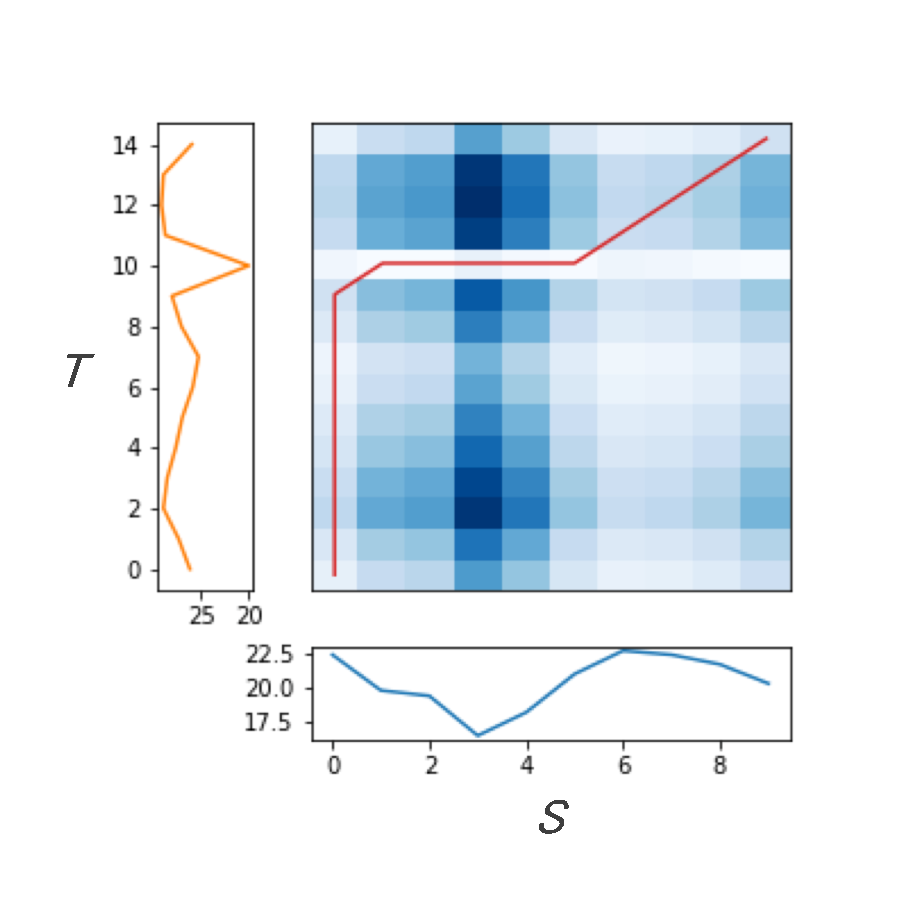
\includegraphics[height=6cm]{dtw.eps}
    \caption{動的時間伸縮法(DTW: Dynamic time warping)の概念図}
    \label{dtw}
\end{figure}

入力と検索対象の各動作の組み合わせで距離を求め,距離が近い動作を入力に類似する動作として抽出する.
距離は0に近いほど類似していることを示し,値が大きくなるほど類似しないことを示す.
次章では,実際に入力を行いDTW距離を算出した結果の分析及びその結果について述べ,
5章で考察を行うことで入力に類した動作を抽出可能な距離について明らかにする.


\chapter{類似動作を抽出可能な距離の分析}

\section{概要}
本章では,入力に類似する動作を抽出可能な距離を明らかにするため,
著者が実装したScratch作品検索システムを用いて複数の入力を行い,
DTW距離の算出結果について定量分析と定性分析を行う.
定量分析では,距離を昇順に並べたある2点の傾きから距離が収束する値を求めることで,
移動方向が全く異なる動作が抽出される距離を明らかにする.
定性分析では,定量分析で明らかにした距離以下の動作を提示し,
動作の類似性を評価するアンケートを実施することで,類似動作を抽出可能な距離を明らかにする.

\section{検索データセット}
\ref{objectbehavior}で述べたように,キー入力やマウス操作などのユーザの操作を必要とするブロックを使用しておらず,
動きブロックを使用している作品に含まれる,
Scratchにデフォルトで用意されている画像を使用したオブジェクトの動作を検索対象とする.
本分析で検索対象外とする作品に使用される,ユーザの操作を必要とするブロックを表\ref{interactionblock}に示す.
Aivaloglouらの公開データセット\cite{dataset}\footnote{https://github.com/TUDelftScratchLab/ScratchDataset}
に含まれる作品の中から条件を満たす13,437件の作品を用いる.

\begin{table}
    \caption{ユーザの操作を必要とするブロック}
    \label{interactionblock}
    \centering
    \begin{tabularx}{\textwidth}{l|l|X}
    \hline
        種類 & ブロック & 説明 \\
        \hline \hline
        \multirow{2}{*}{動きブロック} 
        & マウスポインターへ向ける & オブジェクトの向きをマウスポインターの方向に変更する \\
        \cline{2-3}
        & マウスポインターへ行く & オブジェクトをマウスポインターの位置に動かす \\
        \hline
        \multirow{2}{*}{イベントブロック}
        & (引数)キーが押されたとき & 引数に指定したキーが押された際にスクリプトを実行する \\
        \cline{2-3}
        & このスプライトが押されたとき & オブジェクトがクリックされた際にスクリプトを実行する \\
        \hline
        \multirow{7}{*}{調べるブロック} & マウスポインターに触れた & マウスポインターに触れたことを判定する \\
        \cline{2-3}
        & マウスポインターまでの距離 & オブジェクトとマウスポインター間のユークリッド距離を返す \\
        \cline{2-3}
        & (引数)と聞いて待つ & 引数に指定した文章と共に,画面下部にテキストの入力ボックスを表示する \\
        \cline{2-3}
        & (引数)キーが押された & 指定したキーが押されたことを判定する \\
        \cline{2-3}
        & マウスが押された & マウスが押されたことを判定する \\
        \cline{2-3}
        & マウスのx座標 & 現在のマウスポインターのx座標を返す \\
        \cline{2-3}
        & マウスのy座標 & 現在のマウスポインターのy座標を返す \\
        \hline
    \end{tabularx}
\end{table}

\section{検索システム}
本分析で入力・距離算出を行うために,著者が実装したScratch作品検索システムを用いる.
図\ref{systemdisplay}は検索画面を示す.
図\ref{systemdisplay}の(1)に示すキャンバスにマウス操作で動作のイメージの軌跡を入力し,
検索ボタンをクリックすることで入力と検索対象動作の距離算出を開始する.
全ての動作に対しての距離算出完了後,図\ref{systemdisplay}の(2)に示すように,
「各動作の含まれる作品のURL」「動作を行うスプライトの名称」「入力との距離」を,
距離の昇順に一覧表示する.

\begin{figure}[H]
    \centering
    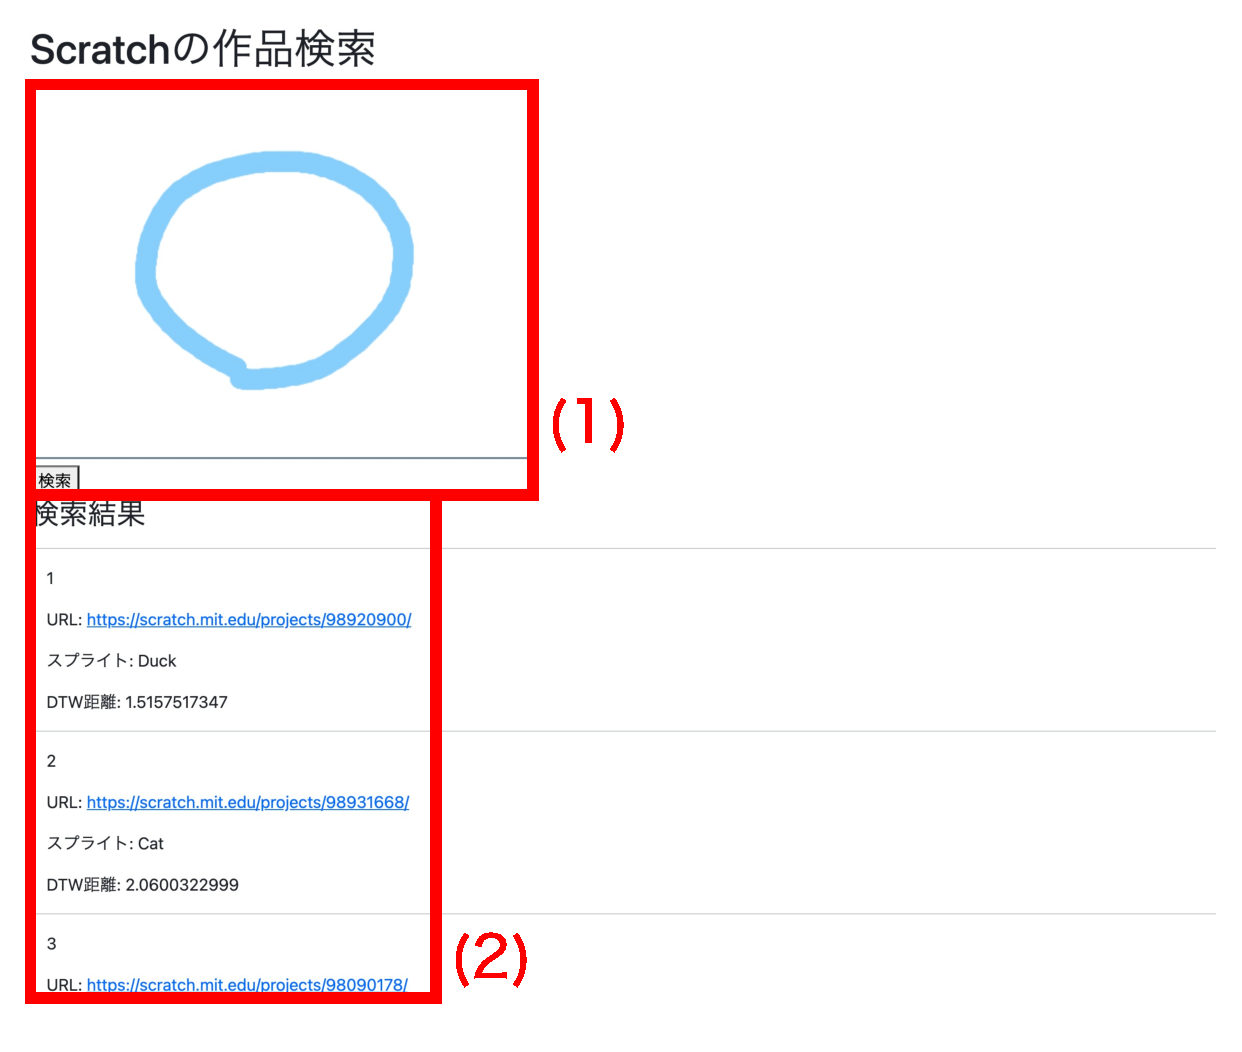
\includegraphics[height=8cm]{systemdisplay.eps}
    \caption{Scratch作品検索システムの画面}
    \label{systemdisplay}
\end{figure}

\section{入力}
Scratchの作品内では,オブジェクトは直線や曲線の移動が行われるため,直線・曲線移動を行う2つの動作を入力する.

\begin{itemize}
    \item 入力a: 左から右へ直線移動(図\ref{input1})
    \item 入力b: 左から上方向へ半円を描く曲線移動(図\ref{input2})
\end{itemize}

以上に加え,より長い動作を入力した場合の距離や動作の類似性についても確認するため,さらに2つの動作を入力する.

\begin{itemize}
    \item 入力c: 左上から時計回りに直線移動(図\ref{input3})
    \item 入力d: 左上から時計回りに曲線移動(図\ref{input4})
\end{itemize}

\begin{figure}[H]
    \centering
    \begin{minipage}{0.2\linewidth}
        \centering
        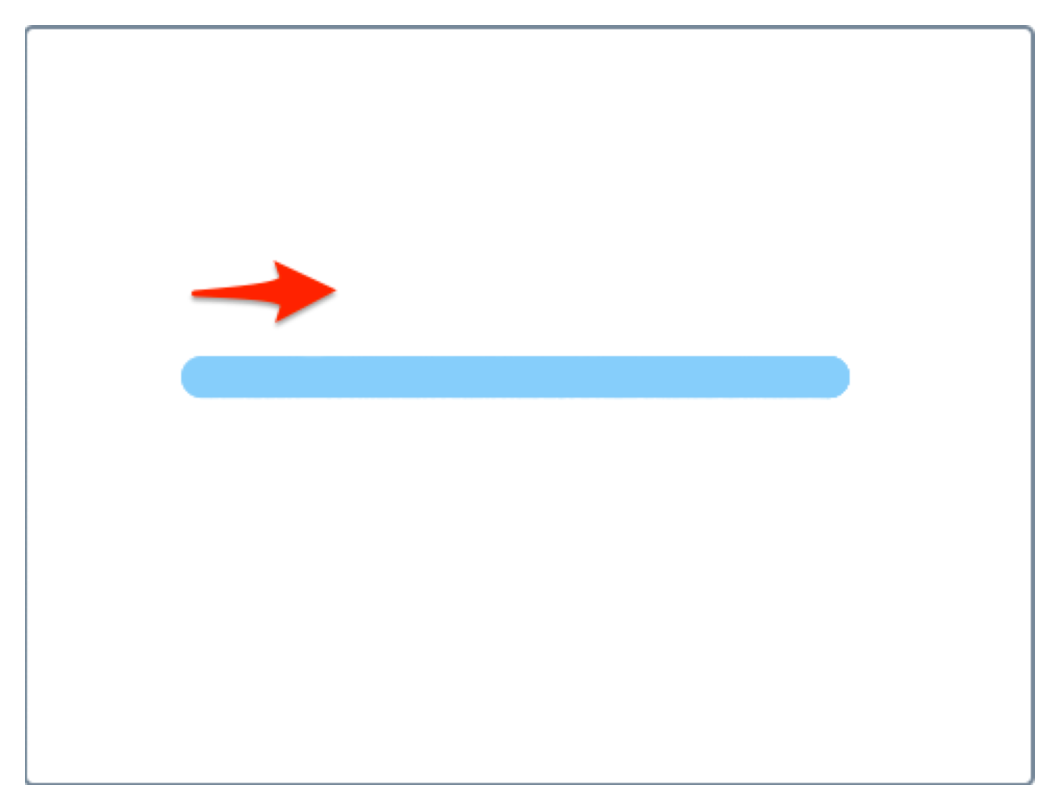
\includegraphics[height=2.5cm]{input1.eps}
        \subcaption{入力a}
        \label{input1}
    \end{minipage}
    \hspace{0.04\columnwidth}
    \begin{minipage}{0.2\linewidth}
        \centering
        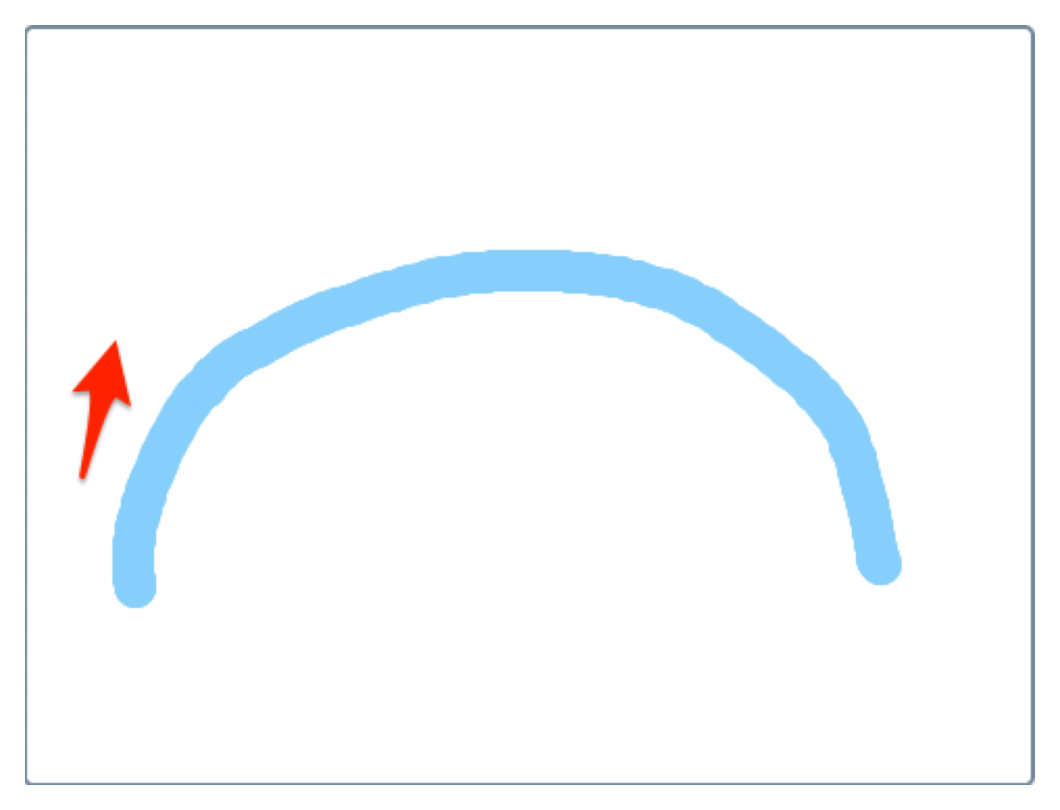
\includegraphics[height=2.5cm]{input2.eps}
        \subcaption{入力b}
        \label{input2}
    \end{minipage}
    \hspace{0.04\columnwidth}
    \begin{minipage}{0.2\linewidth}
        \centering
        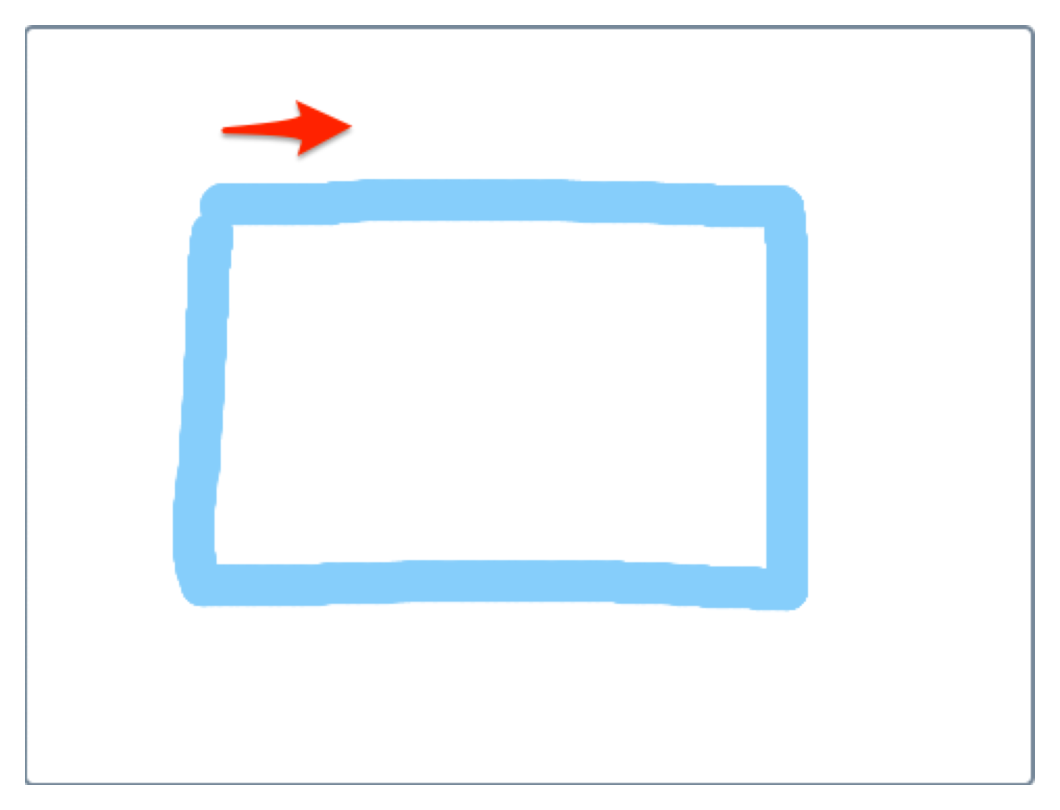
\includegraphics[height=2.5cm]{input3.eps}
        \subcaption{入力c}
        \label{input3}
    \end{minipage}
    \hspace{0.04\columnwidth}
    \begin{minipage}{0.2\linewidth}
        \centering
        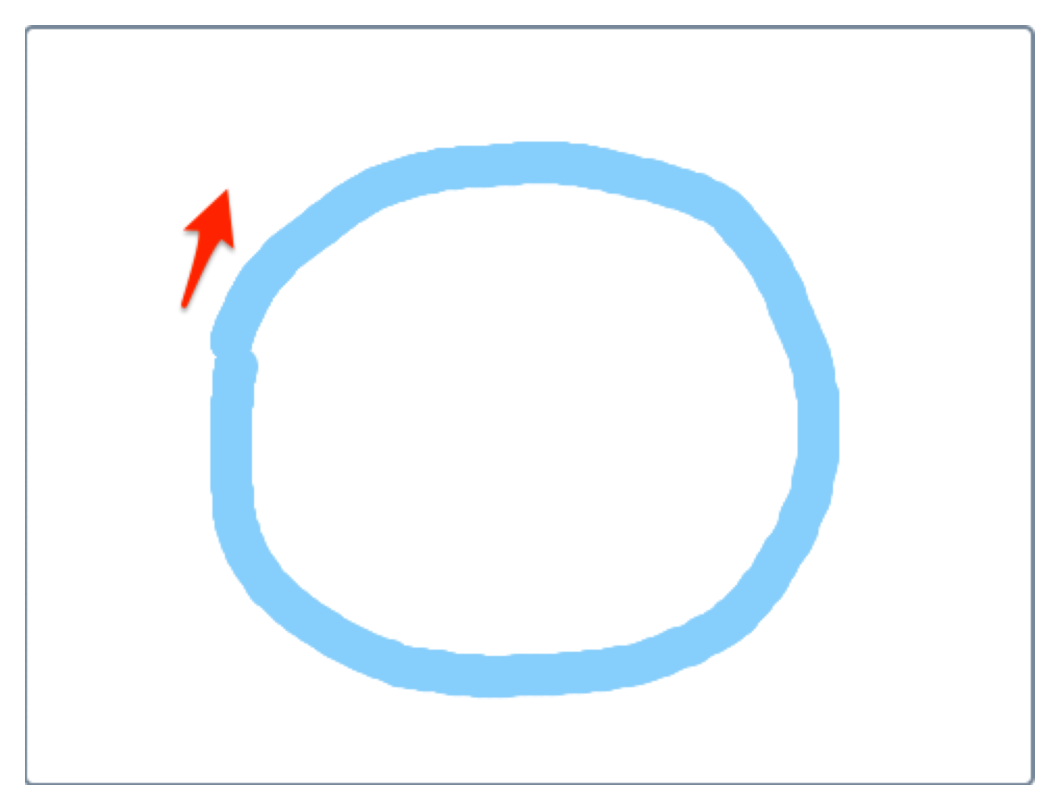
\includegraphics[height=2.5cm]{input4.eps}
        \subcaption{入力d}
        \label{input4}
    \end{minipage}
    \caption{分析で用いる4つの入力}
    \label{analyticsinput}
\end{figure}

\section{定量分析}
定量分析では,移動方向が全く異なる動作が抽出される距離を明らかにするために,
距離を昇順に並べたある2点の傾きから距離が収束する値を求める.
距離が収束する値は次に示す手順で求める.

\begin{enumerate}
    \item 距離が近い動作から50件ごとに傾きを算出
    \item 傾きが0.5を切る距離の動作のスナップショットを目視で確認
    \item 2の結果,入力と類似しない動作であった場合,その距離以下の動作を提示
    ただし,データセット数が多いため,各動作の距離を小数点第2位で四捨五入した値が重複する動作を削除
    \item 2の結果,入力と類似する動作であった場合,2以降の手順を再度行う
\end{enumerate}

各入力に対して定量分析を行なった結果を表\ref{quantitativeresult}に示す.
定量分析で明らかにした距離は,\ref{teisei}の定性分析で実施するアンケートに提示する動作の抽出に用いる.
        
\begin{table}[H]
    \caption{移動方向が全く異なる動作が抽出される距離}
    \label{quantitativeresult}
    \centering
    \begin{tabular}{c|c}
    \hline
    入力 & 距離 \\
    \hline \hline
    a & 4.4 \\
    \hline
    b & 3.2 \\
    \hline
    c & 6.9 \\
    \hline
    d & 7.9 \\
    \hline
    \end{tabular}
\end{table}


\section{定性分析}
\label{teisei}
定性分析では,入力に類似する動作を抽出可能な距離を明らかにするために,
入力と各検索対象動作のDTW距離算出結果から距離の異なる複数の動作を提示し,動作の類似性をアンケートで評価する.

提示された動作が,入力と類似するかどうかを判断するために,次の1つ目の質問を設けた.

\begin{itemize}
    \item 質問1: スナップショットの動作は,入力に類似していますか?
\end{itemize}

質問1に対して,4段階のリッカート尺度(1: 類似する,2: やや類似する,3: やや類似しない,4: 類似しない)で評価を行う.
初めてアンケートの回答者全員が「4: 類似しない」を選択した距離を,
本分析で明らかにする類似動作を抽出可能な距離とする.
また,回答者にとってどのような理由で評価に繋がるかについて明らかにするために,
「1: 類似する」以外を選択した場合の理由を記述してもらった.

さらに,本研究は他者のプログラムを参照することによる学習の支援を期待するため,
提示された動作のプログラムを参考に入力と類似する動作を実装できるかについて判断する2つ目の質問を設けた.

\begin{itemize}
    \item 質問2: プログラムを参考に入力と同じ動きを実装できますか?
\end{itemize}

質問2に対して,2値(1: 実装できる,2: 実装できない) で評価を行う.
アンケートの回答結果から,「動作は類似するがプログラムは参考にならない」
「動作は類似しないがプログラムは参考になる」といった事例の調査と考察を行うことで,
本研究が与え得る他者のプログラムを参照することによる学習への影響を明らかにする.

アンケートはプログラムの理解が必要であるため,Scratchのプログラムを理解できる著者を含む3人が回答した.

\subsubsection{入力a}
入力aのアンケート結果を表\ref{resulta}に示す.
最も近い距離0.3\footnote{https://scratch.mit.edu/projects/99901051/}から
距離0.8\footnote{https://scratch.mit.edu/projects/98351336/}の動作までは,
質問1は「類似する」を,質問2は「実装できる」を全員が選択した.
距離0.9\footnote{https://scratch.mit.edu/projects/98971685/}の動作で,
質問2の「実装できない」を初めて1人の回答者が選択した.
「実装できない」を選択した回答者は,
距離0.9の動作はプログラムはオブジェクトの向いている方向に進む「(引数)歩動かす」ブロックを用いているが,
オブジェクトが向いている方向が左に初期化されているため,右方向の移動は実装できないと判断した.
一方「実装できる」を選択した回答者は,
オブジェクトの向きを右に初期化すれば,プログラムを参考に右方向の移動を実装できると判断した.
質問1に対して全員が「類似する」を選択した動作は
距離1.6\footnote{https://scratch.mit.edu/projects/95056796/}まで続くが,
距離1.7\footnote{https://scratch.mit.edu/projects/99094173/}以降で「やや類似する」を選択した動作が出現している.
距離1.7の動作で「やや類似する」を選択した回答者は,移動距離が短すぎることから「やや類似する」と判断した.
また,距離2.2\footnote{https://scratch.mit.edu/projects/98073088/}の動作で,
質問1の「やや類似しない」を初めて1人の回答者が選択した.
距離2.2の動作は横方向に往復する動作であり,「やや類似しない」を選択した回答者は,
右方向への移動を含んでいるが,往復をしているため直感的に類似しないと判断した.
距離4.3\footnote{https://scratch.mit.edu/projects/98964270/}の動作は,
質問1で「やや類似しない」を初めて回答者全員が選択した.
距離4.3の動作は右方向に進んでいるがやや上方向の移動も含んでおり,
「やや類似しない」を選択した理由として,上方向の移動が含まれていることを回答者全員が述べている.
質問2に対しては2人が「実装できない」を,1人が「実装できる」を選択している.
この動作のプログラムは,座標を指定することでオブジェクトを移動させる
「(引数)秒でx座標を(引数)に,y座標を(引数)に変える」ブロックを用いており,
「実装できる」を選択した回答者は,オブジェクトのy座標が変化しないよう引数を指定することで実装できると述べている.
距離4.4\footnote{https://scratch.mit.edu/projects/99096873/}の動作で
初めて全員が質問1の「類似しない」を選択した.
距離4.4の動作は,該当する画像を用いたオブジェクトが3つ存在しており,
どのオブジェクトが動作の対象であるかわからないことや,スナップショット内に右方向への移動を含んでいないことから
「類似しない」が選択された.
質問2では2人が「実装できる」を,1人が「実装できない」を選択した.
「実装できる」を選択した理由として,3つのうち1つのオブジェクトで「(引数)歩動かす」ブロックを用いており,
オブジェクトの向きを右に初期化すれば,右方向の移動を実装できるとしている.
初めて回答者全員が「類似しない」を選択した距離は4.4であるため,
類似動作を抽出可能な距離は4.3\footnote{https://scratch.mit.edu/projects/98964270/}以下となる.

\subsubsection{入力b}
入力bのアンケート結果を表\ref{resultb}に示す.
最も近い距離0.9\footnote{https://scratch.mit.edu/projects/99730968/}から
距離1.2\footnote{https://scratch.mit.edu/projects/99730486/}の動作まで,
回答者全員が質問1で「類似する」を,質問2で「実装できる」を選択した.
距離1.3\footnote{https://scratch.mit.edu/projects/95814344/}の動作は,
質問1で「やや類似する」が選択されている.
「やや類似する」を選択した理由として,回答者は大きい円の一部に見えたとしている.
距離1.4\footnote{https://scratch.mit.edu/projects/99912783/}の動作は,
質問1で「類似する」あるいは「やや類似する」を選択したが,
質問2で「実装できない」を回答者全員が選択した.
動作の見た目は類似するように見えるが,プログラムを見ると曲線移動ではなく直線移動をしているため,
このような結果となった.
距離1.6\footnote{https://scratch.mit.edu/projects/95814344/}の動作では,
初めて質問1の「類似しない」が選択された.
「類似しない」を選択した理由は,入力のようなゆるやかな半円でなく,急角度の半円であるためとしている.
以降の距離で「類似する」「やや類似する」を選択しているが,
回答者によっては「やや類似しない」や「類似しない」を選択している.
距離2.2\footnote{https://scratch.mit.edu/projects/99822646/}の動作で初めて全員が質問1の「類似しない」を選択した.
距離2.2\footnote{https://scratch.mit.edu/projects/99822646/}の動作は右下へ直線移動をする動作であり,
半円とは全く異なる動きをしているために全員が「類似しない」を選択した.
質問2についても.全員が「実装できない」を選択した.
以降の距離で,「やや類似する」が登場しながらもほとんどが「やや類似しない」「類似しない」を占めており,
距離2.8\footnote{https://scratch.mit.edu/projects/99473659/}以上の全ての動作で,
全員が「類似しない」を選択した.
初めて回答者全員が「類似しない」を選択した距離は2.2であるため,
類似動作を抽出可能な距離は2.1\footnote{https://scratch.mit.edu/projects/99581277/}以下となる.

\subsubsection{入力c}
入力cのアンケート結果を表\ref{resultc}に示す.
最も距離の近い1.7\footnote{https://scratch.mit.edu/projects/98914463/}の動作に対して,
全員が質問1の「やや類似する」を選択した.
「やや類似する」を選択した理由として,距離1.7の動作は四角形を描いているが,ある辺が斜めに描かれていることから,
入力のような真っ直ぐの辺を描くものではないとしている.
距離2.6\footnote{https://scratch.mit.edu/projects/96431586/}の動作で
初めて質問1の「やや類似しない」が選択された.
この動作は角度を変えながら壁に跳ね返るプログラムで四角形が描かれているように見えるが,
入力のような真っ直ぐの辺を描くものではないため
「やや類似しない」が選択された.
四角形を描くためのプログラムではないため,質問2では全員が「実装できない」を選択している.
距離3.7\footnote{https://scratch.mit.edu/projects/98149958/}から
4.0\footnote{https://scratch.mit.edu/projects/98149958/}までの動作は,
全て同じ作品に含まれる動作で,1人が「やや類似しない」を選択した.
「やや類似しない」を選択した理由は,いずれの動作も,最初の右方向の一辺の移動が含まれていないためである.
しかし,プログラムは四角形を描くものとなっており,質問2では全員が「実装できる」を選択している.
距離4.1\footnote{https://scratch.mit.edu/projects/99394518/}の動作で初めて全員が「類似しない」を選択した.
「類似しない」を選択した理由は,四角形ではなく円の一部を描くためである.
質問2においても,全員が「実装できない」を選択した.
以降の距離で,「類似する」「やや類似する」が登場しながらもほとんどが「やや類似しない」「類似しない」を占めている.
初めて回答者全員が「類似しない」を選択した距離は4.1であるため,
類似動作を抽出可能な距離は4.0\footnote{https://scratch.mit.edu/projects/98149958/}以下となる.

\subsubsection{入力d}
入力dのアンケート結果を表\ref{resultd}に示す.
全員が「類似する」を選択した動作は,
最も距離の近い1.7\footnote{https://scratch.mit.edu/projects/99617573/}の動作のみである.
2番目に距離の近い3.2\footnote{https://scratch.mit.edu/projects/99039933/}の動作では.
2人が「やや類似しない」を,1人が「類似しない」を選択した.
この動作は.移動方向は類似しているが,円ではなく四角形を描いているため
「やや類似しない」あるいは「類似しない」が選択された.
以降の全ての動作で1人は「やや類似しない」あるいは「類似しない」を選択している.
距離4.5\footnote{https://scratch.mit.edu/projects/97152443/}の動作で,初めて全員が「類似しない」を選択した.
この動作も円ではなく四角形を描いているため,「類似しない」が選択された.
以降の距離で,「類似する」「やや類似する」が登場しながらもほとんどが「やや類似しない」「類似しない」を占めている.
初めて回答者全員が「類似しない」を選択した距離は4.5であるため,
類似動作を抽出可能な距離は4.4\footnote{https://scratch.mit.edu/projects/98876669/}以下となる.

\begin{table}
    \caption{入力aのアンケート結果}
    \label{resulta}
    \centering
    \scalebox{0.8}{
    \begin{tabular}{c|c|c|c|c|c|c}
    \hline
     & \multicolumn{4}{c|}{質問1の回答数} & \multicolumn{2}{c}{質問2の回答数} \\
    \hline
    距離 & 1: 類似する & 2: やや類似する & 3: やや類似しない & 4: 類似しない & 1: 実装できる & 2: 実装できない \\
    \hline \hline
    0.3 & 3 & 0 & 0 & 0 & 3 & 0 \\
    \hline
    0.4 & 3 & 0 & 0 & 0 & 3 & 0 \\
    \hline
    0.5 & 3 & 0 & 0 & 0 & 3 & 0 \\
    \hline
    0.6 & 3 & 0 & 0 & 0 & 3 & 0 \\
    \hline
    0.7 & 3 & 0 & 0 & 0 & 3 & 0 \\
    \hline
    0.8 & 3 & 0 & 0 & 0 & 3 & 0 \\
    \hline
    0.9 & 3 & 0 & 0 & 0 & 2 & 1 \\
    \hline
    1.0 & 3 & 0 & 0 & 0 & 2 & 1 \\
    \hline
    1.1 & 3 & 0 & 0 & 0 & 3 & 0 \\
    \hline
    1.2 & 3 & 0 & 0 & 0 & 2 & 1 \\
    \hline
    1.3 & 3 & 0 & 0 & 0 & 3 & 0 \\
    \hline
    1.4 & 3 & 0 & 0 & 0 & 3 & 0 \\
    \hline
    1.5 & 3 & 0 & 0 & 0 & 3 & 0 \\
    \hline
    1.6 & 3 & 0 & 0 & 0 & 3 & 0 \\
    \hline
    1.7 & 2 & 1 & 0 & 0 & 3 & 0 \\
    \hline
    1.8 & 3 & 0 & 0 & 0 & 3 & 0 \\
    \hline
    1.9 & 3 & 0 & 0 & 0 & 3 & 0 \\
    \hline
    2.0 & 2 & 1 & 0 & 0 & 3 & 0 \\
    \hline
    2.1 & 2 & 1 & 0 & 0 & 3 & 0 \\
    \hline
    2.2 & 2 & 0 & 1 & 0 & 2 & 1 \\
    \hline
    2.3 & 3 & 0 & 0 & 0 & 3 & 0 \\
    \hline
    2.4 & 1 & 1 & 1 & 0 & 3 & 0 \\
    \hline
    2.5 & 3 & 0 & 0 & 0 & 3 & 0 \\
    \hline
    2.6 & 2 & 0 & 1 & 0 & 3 & 0 \\
    \hline
    2.7 & 3 & 0 & 0 & 0 & 3 & 0 \\
    \hline
    2.8 & 3 & 0 & 0 & 0 & 3 & 0 \\
    \hline
    2.9 & 3 & 0 & 0 & 0 & 3 & 0 \\
    \hline
    3.0 & 0 & 3 & 0 & 0 & 3 & 0 \\
    \hline
    3.1 & 3 & 0 & 0 & 0 & 3 & 0 \\
    \hline
    3.2& 2 & 0 & 0 & 1 & 1 & 2 \\
    \hline
    3.3 & 3 & 0 & 0 & 0 & 3 & 0 \\
    \hline
    3.4 & 1 & 0 & 2 & 0 & 3 & 0 \\
    \hline
    3.5 & 3 & 0 & 0 & 0 & 2 & 1 \\
    \hline
    3.6 & 3 & 0 & 0 & 0 & 3 & 0 \\
    \hline
    3.7 & 1 & 0 & 2 & 0 & 2 & 1 \\
    \hline
    3.8 & 3 & 0 & 0 & 0 & 3 & 0 \\
    \hline
    3.9 & 2 & 1 & 0 & 0 & 3 & 0 \\
    \hline
    4.0 & 0 & 1 & 2 & 0 & 3 & 0 \\
    \hline
    4.1 & 3 & 0 & 0 & 0 & 3 & 0 \\
    \hline
    4.2 & 3 & 0 & 0 & 0 & 3 & 0 \\
    \hline
    4.3 & 0 & 0 & 3 & 0 & 1 & 2 \\
    \hline
    4.4 & 0 & 0 & 0 & 3 & 2 & 1 \\
    \hline
    \end{tabular}
    }
\end{table}

\begin{table}
    \caption{入力bのアンケート結果}
    \label{resultb}
    \centering
    \scalebox{0.8}{
    \begin{tabular}{c|c|c|c|c|c|c}
    \hline
     & \multicolumn{4}{c|}{質問1の回答数} & \multicolumn{2}{c}{質問2の回答数} \\
    \hline
    距離 & 1: 類似する & 2: やや類似する & 3: やや類似しない & 4: 類似しない & 1: 実装できる & 2: 実装できない \\
    \hline \hline
    0.9 & 3 & 0 & 0 & 0 & 3 & 0 \\
    \hline
    1.2 & 3 & 0 & 0 & 0 & 3 & 0 \\
    \hline
    1.3 & 2 & 1 & 0 & 0 & 2 & 1 \\
    \hline
    1.4 & 2 & 1 & 0 & 0 & 0 & 3 \\
    \hline
    1.5 & 2 & 1 & 0 & 0 & 1 & 2 \\
    \hline
    1.6 & 1 & 1 & 0 & 1 & 1 & 2 \\
    \hline
    1.7 & 1 & 2 & 0 & 0 & 1 & 2 \\
    \hline
    1.8 & 2 & 1 & 0 & 0 & 1 & 2 \\
    \hline
    1.9 & 1 & 1 & 0 & 1 & 1 & 2 \\
    \hline
    2.0 & 1 & 2 & 0 & 0 & 0 & 3 \\
    \hline
    2.1 & 2 & 0 & 1 & 0 & 2 & 1 \\
    \hline
    2.2 & 0 & 0 & 0 & 3 & 0 & 3 \\
    \hline
    2.3 & 0 & 2 & 0 & 1 & 1 & 2 \\
    \hline
    2.4 & 0 & 0 & 1 & 2 & 0 & 3 \\
    \hline
    2.5 & 0 & 1 & 2 & 0 & 0 & 3 \\
    \hline
    2.6 & 0 & 0 & 0 & 3 & 0 & 3 \\
    \hline
    2.7 & 0 & 0 & 3 & 0 & 0 & 3 \\
    \hline
    2,8 & 0 & 0 & 0 & 3 & 0 & 3 \\
    \hline
    2.9 & 0 & 0 & 0 & 3 & 0 & 3 \\
    \hline
    3.0 & 0 & 0 & 0 & 3 & 0 & 3 \\
    \hline
    3.1 & 0 & 0 & 0 & 3 & 0 & 3 \\
    \hline
    3.2 & 0 & 0 & 0 & 3 & 0 & 3 \\
    \hline
    \end{tabular}
    }
\end{table}

\begin{table}
    \caption{入力cのアンケート結果}
    \label{resultc}
    \centering
    \scalebox{0.8}{
    \begin{tabular}{c|c|c|c|c|c|c}
    \hline
     & \multicolumn{4}{c|}{質問1の回答数} & \multicolumn{2}{c}{質問2の回答数} \\
    \hline
    距離 & 1: 類似する & 2: やや類似する & 3: やや類似しない & 4: 類似しない & 1: 実装できる & 2: 実装できない \\
    \hline \hline
    1.7 & 0 & 3 & 0 & 0 & 3 & 0 \\
    \hline
    2.2 & 3 & 0 & 0 & 0 & 3 & 0 \\
    \hline
    2.6 & 0 & 2 & 1 & 0 & 0 & 3 \\
    \hline
    3.0 & 3 & 0 & 0 & 0 & 3 & 0 \\
    \hline
    3.3 & 2 & 1 & 0 & 0 & 3 & 0 \\
    \hline
    3.7 & 2 & 0 & 1 & 0 & 3 & 0 \\
    \hline
    3.8 & 2 & 0 & 1 & 0 & 0 & 3 \\
    \hline
    3.9 & 1 & 1 & 1 & 0 & 3 & 0 \\
    \hline
    4.0 & 1 & 1 & 0 & 1 & 1 & 2 \\
    \hline
    4.1 & 0 & 0 & 0& 3 & 0 & 3 \\
    \hline
    4.3 & 0 & 0 & 0& 3 & 0 & 3 \\
    \hline
    4.4 & 0 & 0 & 0 & 3 & 0 & 3 \\
    \hline
    4.5 & 2 & 1 & 0 & 0 & 3 & 0 \\
    \hline
    4.6 & 0 & 0 & 1 & 2 & 1 & 2 \\
    \hline
    4.7 & 1 & 1 & 1 & 0 & 2 & 1 \\
    \hline
    4.8 & 0 & 0 & 2 & 1 & 2 & 1 \\
    \hline
    4.9 & 1 & 0 & 1 & 0 & 0 & 3 \\
    \hline
    5.0 & 0 & 1 & 2 & 0 & 3 & 0 \\
    \hline
    5.1 & 0 & 0 & 0 & 3 & 0 & 3 \\
    \hline
    5.2 & 0 & 0 & 2 & 1 & 1 & 2 \\
    \hline
    5.3 & 0 & 0 & 0 & 3 & 1 & 2 \\
    \hline
    5.4 & 0 & 0 & 0 & 3 & 0 & 3 \\
    \hline
    5.4 & 0 & 0 & 0 & 3 & 0 & 3 \\
    \hline
    5.5 & 1 & 2 & 0 & 0 & 3 & 0 \\
    \hline
    5.6 & 1 & 2 & 0 & 0 & 3 & 0 \\
    \hline
    5.7 & 0 & 1 & 2 & 0 & 2 & 1 \\
    \hline
    5.8 & 0 & 0 & 1 & 2 & 0 & 3 \\
    \hline
    5.9 & 0 & 1 & 2 & 0 & 1 & 2 \\
    \hline
    6.0 & 0 & 0 & 0 & 3 & 0 & 3 \\
    \hline
    6.1 & 0 & 0 & 0 & 3 & 0 & 3 \\
    \hline
    6.2 & 0 & 0 & 0 & 3 & 0 & 3 \\
    \hline
    6.3 & 0 & 0 & 0 & 3 & 0 & 3 \\
    \hline
    6.4 & 0 & 0 & 0 & 3 & 0 & 3 \\
    \hline
    6.5 & 0 & 0 & 0 & 3 & 1 & 2 \\
    \hline
    6.6 & 0 & 0 & 0 & 3 & 0 & 3 \\
    \hline
    6.7 & 0 & 0 & 0 & 3 & 0 & 3 \\
    \hline
    6.8 & 2 & 0 & 1 & 0 & 2 & 1 \\
    \hline
    6.9 & 0 & 0 & 0 & 3 & 0 & 3 \\
    \hline
    \end{tabular}
    }
\end{table}          

\begin{table}
    \caption{入力dのアンケート結果}
    \label{resultd}
    \centering
    \scalebox{0.8}{
    \begin{tabular}{c|c|c|c|c|c|c}
    \hline
     & \multicolumn{4}{c|}{質問1の回答数} & \multicolumn{2}{c}{質問2の回答数} \\
    \hline
    距離 & 1: 類似する & 2: やや類似する & 3: やや類似しない & 4: 類似しない & 1: 実装できる & 2: 実装できない \\
    \hline \hline
    1.7 & 3 & 0 & 0 & 0 & 3 & 0 \\
    \hline
    3.2 & 0 & 0 & 2 & 1 & 0 & 3 \\
    \hline
    4.3 & 0 & 0 & 1 & 2 & 1 & 2 \\
    \hline
    4.4 & 0 & 2 & 0 & 1 & 3 & 0\\
    \hline
    4.5 & 0 & 0 & 0 & 3 & 1 & 2 \\
    \hline
    4.6 & 0 & 0 & 0 & 3 & 1 & 2 \\
    \hline
    4.7 & 0 & 0 & 0 & 3 & 0 & 3 \\
    \hline
    4.8 & 0 & 0 & 2 & 1 & 0 & 3 \\
    \hline
    5.0 & 0 & 0 & 0& 3 & 0 & 3 \\
    \hline
    5.1 & 0 & 2 & 0& 1 & 3 & 0 \\
    \hline
    5.2 & 0 & 1 & 1& 1 & 3 & 0 \\
    \hline
    5.3 & 0 & 1 & 2 & 0 & 1 & 2 \\
    \hline
    5.4 & 0 & 2 & 0 & 1 & 3 & 0 \\
    \hline
    5.5 & 0 & 2 & 1 & 0 & 2 & 1 \\
    \hline
    5.6 & 0 & 1 & 1 & 1 & 3 & 0 \\
    \hline
    5.9 & 0 & 1 & 1 & 1 & 3 & 0 \\
    \hline
    6.0 & 0 & 0 & 0 & 3 & 1 & 2 \\
    \hline
    6.1 & 0 & 0 & 0 & 3 & 0 & 3 \\
    \hline
    6.2 & 0 & 2 & 0 & 1 & 3 & 0 \\
    \hline
    6.3 & 0 & 0 & 0 & 3 & 1 & 2 \\
    \hline
    6.4 & 0 & 2 & 0 & 1 & 3 & 0 \\
    \hline
    6.5 & 0 & 0 & 0 & 3 & 0 & 3 \\
    \hline
    6.6 & 0 & 1 & 1 & 1 & 1 & 2 \\
    \hline
    6.8 & 0 & 0 & 0 & 3 & 0 & 3 \\
    \hline
    6.9 & 0 & 0 & 0 & 3 & 0 & 3 \\
    \hline
    7.0 & 0 & 0 & 0 & 3 & 0 & 3 \\
    \hline
    7.1 & 0 & 0 & 1 & 2 & 1 & 2 \\
    \hline
    7.2 & 0 & 0 & 0 & 3 & 0 & 3 \\
    \hline
    7.3 & 0 & 2 & 0 & 1 & 1 & 2 \\
    \hline
    7.4 & 0 & 2 & 0 & 1 & 3 & 0 \\
    \hline
    7.5 & 0 & 0 & 0 & 3 & 0 & 3 \\
    \hline
    7.6 & 0 & 0 & 0 & 3 & 1 & 2 \\
    \hline
    7.7 & 0 & 0 & 1 & 2 & 1 & 2 \\
    \hline
    7.8 & 0 & 0 & 0 & 3 & 0 & 3 \\
    \hline
    7.9 & 0 & 0 & 0 & 3 & 1 & 2 \\
    \hline
    \end{tabular}
    }
\end{table}       


\chapter{考察}
本章では,類似動作を抽出可能な距離の考察を述べる.

\section{定量分析}

\section{定性分析}
\subsection{動作の類似性と距離}
入力aから入力dまで,類似動作を抽出可能な距離は異なる結果となった.
特に入力bは,他の3つの入力の距離の最大値が4台であるのに対し,約半分の2.1であった.
入力は無数のパターンが存在するため,それら全てに
類似動作を抽出可能な距離を決定することは不可能である.
このことから,検索結果の動作を距離を一意に決めてその距離以下の動作を提示するのではなく,
近いもの順に全て提示することが良いと思われる.
ただし,全く類似しない動作が連続して提示されることを防ぐために,
4章で行った動作の足切りを行うのは良いと考える.

曲線移動を検索したとしても,変化の具合が似ていると直線移動の動作が抽出されることもある.
その逆のパターンも存在している.
曲線移動と直線移動の区別を行うためには,
入力や検索対象動作の座標変化をより細かい間隔で取得する必要があると考える.

反転したオブジェクト画像の認識はできない.
画像認識のテンプレート画像として,反転したオブジェクト画像も用意する必要があることがわかった.

\subsection{プログラムの多様性}
アンケートで提示した動作の中に,プログラムの多様性が見られた.
入力aを例に挙げると,

\section{より長い動作の検索}
4章の分析で用いた入力よりもさらに長い動作を検索可能かどうかを明らかにするために,
追加で図\ref{considerinput}に示す2つの入力を行い,4章と同様のアンケートを実施した.
アンケートに提示する動作は,4章と同様の手順で抽出した.

\begin{figure}[H]
    \centering
    \begin{minipage}{0.2\linewidth}
        \centering
        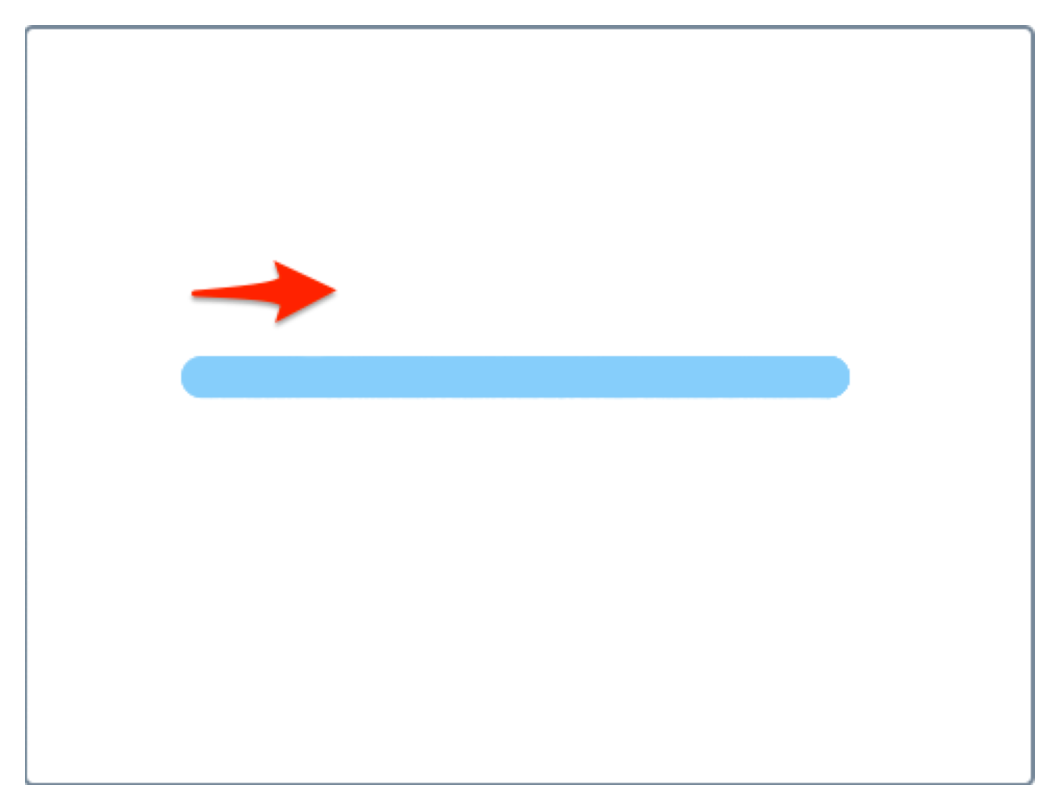
\includegraphics[height=2.5cm]{input1.eps}
        \subcaption{入力e}
        \label{input5}
    \end{minipage}
    \hspace{0.04\columnwidth}
    \begin{minipage}{0.2\linewidth}
        \centering
        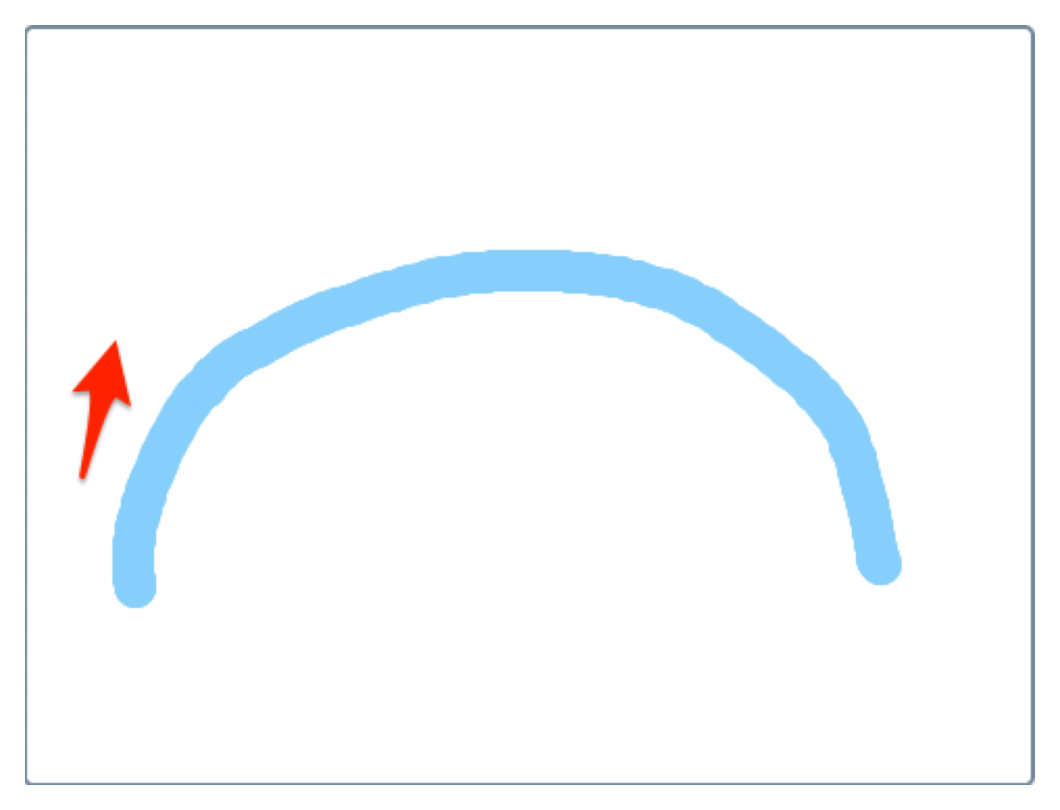
\includegraphics[height=2.5cm]{input2.eps}
        \subcaption{入力f}
        \label{input6}
    \end{minipage}
    \hspace{0.04\columnwidth}
    \caption{追加で行う2つの入力}
    \label{considerinput}
\end{figure}

入力eのアンケート結果を表\ref{resulte}に示す.

入力fのアンケート結果を表\ref{resultf}に示す.

\begin{table}
    \caption{入力eのアンケート結果}
    \label{resulte}
    \centering
    \scalebox{0.8}{
    \begin{tabular}{c|c|c|c|c|c|c}
    \hline
     & \multicolumn{4}{c|}{質問1の回答数} & \multicolumn{2}{c}{質問2の回答数} \\
    \hline
    距離 & 1: 類似する & 2: やや類似する & 3: やや類似しない & 4: 類似しない & 1: 実装できる & 2: 実装できない \\
    \hline \hline
    4.0 & 3 & 0 & 0 & 0 & 3 & 0 \\
    \hline
    9.2 & 0 & 0 & 0 & 3 & 1 & 2 \\
    \hline
    9.9 & 0 & 0 & 0 & 3 & 0 & 3 \\
    \hline
    10.3 & 0 & 0 & 0 & 3 & 0 & 3 \\
    \hline
    10.5 & 0 & 0 & 0 & 3 & 0 & 3 \\
    \hline
    10.6 & 0 & 0 & 0 & 3 & 0 & 3 \\
    \hline
    10.7 & 0 & 0 & 0 & 3 & 0 & 3 \\
    \hline
    10.8 & 0 & 0 & 0 & 3 & 0 & 3 \\
    \hline
    11.2 & 0 & 0 & 0 & 3 & 0 & 3 \\
    \hline
    11.3 & 0 & 0 & 0 & 3 & 1 & 2 \\
    \hline
    11.4 & 0 & 0 & 0 & 3 & 0 & 3 \\
    \hline
    11.5 & 0 & 0 & 0 & 3 & 1 & 2 \\
    \hline
    11.6 & 0 & 0 & 0 & 3 & 1 & 2 \\
    \hline
    11.8 & 0 & 0 & 0 & 3 & 1 & 2 \\
    \hline
    11.9 & 0 & 0 & 0 & 3 & 0 & 3 \\
    \hline
    12.0 & 0 & 0 & 0 & 3 & 0 & 3 \\
    \hline
    12.1 & 0 & 0 & 0 & 3 & 0 & 3 \\
    \hline
    12.2 & 0 & 0 & 0 & 3 & 1 & 2 \\
    \hline
    12.3 & 0 & 0 & 0 & 3 & 0 & 3 \\
    \hline
    12.4 & 0 & 0 & 0 & 3 & 0 & 3 \\
    \hline
    12.5 & 0 & 0 & 0 & 3 & 1 & 2 \\
    \hline
    12.6 & 0 & 0 & 0 & 3 & 1 & 2 \\
    \hline
    12.7 & 0 & 0 & 0 & 3 & 0 & 3 \\
    \hline
    12.8 & 0 & 0 & 0 & 3 & 1 & 2 \\
    \hline
    12.9 & 0 & 0 & 0 & 3 & 0 & 3 \\
    \hline
    13.0 & 0 & 0 & 0 & 3 & 1 & 2 \\
    \hline
    13.1 & 0 & 0 & 0 & 3 & 0 & 3 \\
    \hline
    13.2 & 0 & 0 & 0 & 3 & 0 & 3 \\
    \hline
    13.4 & 0 & 0 & 0 & 3 & 1 & 2 \\
    \hline
    13.5& 0 & 0 & 0 & 3 & 1 & 2 \\
    \hline
    13.6 & 0 & 0 & 0 & 3 & 0 & 3 \\
    \hline
    13.7 & 0 & 0 & 0 & 3 & 1 & 2 \\
    \hline
    13.8 & 0 & 0 & 0 & 3 & 1 & 2 \\
    \hline
    13.9 & 0 & 0 & 0 & 3 & 1 & 2 \\
    \hline
    14.0 & 0 & 0 & 0 & 3 & 0 & 3 \\
    \hline
    14.1 & 0 & 0 & 0 & 3 & 1 & 2 \\
    \hline
    14.2 & 0 & 0 & 0 & 3 & 0 & 3 \\
    \hline
    14.3 & 0 & 0 & 0 & 3 & 0 & 2 \\
    \hline
    \end{tabular}
    }
\end{table}

\begin{table}
    \caption{入力fのアンケート結果}
    \label{resultf}
    \centering
    \scalebox{0.8}{
    \begin{tabular}{c|c|c|c|c|c|c}
    \hline
     & \multicolumn{4}{c|}{質問1の回答数} & \multicolumn{2}{c}{質問2の回答数} \\
    \hline
    距離 & 1: 類似する & 2: やや類似する & 3: やや類似しない & 4: 類似しない & 1: 実装できる & 2: 実装できない \\
    \hline \hline
    4.5 & 0 & 1 & 2 & 0 & 1 & 2 \\
    \hline
    6.7 & 1 & 1 & 0 & 1 & 2 & 1 \\
    \hline
    6.8 & 0 & 0 & 2 & 1 & 0 & 3 \\
    \hline
    6.9 & 0 & 0 & 0 & 3 & 0 & 3 \\
    \hline
    7.1 & 0 & 0 & 1 & 2 & 0 & 3 \\
    \hline
    7.3 & 0 & 0 & 0 & 3 & 0 & 3 \\
    \hline
    7.4 & 0 & 0 & 0 & 3 & 0 & 3 \\
    \hline
    7.5 & 0 & 0 & 0 & 3 & 0 & 3 \\
    \hline
    7.6 & 0 & 0 & 1 & 2 & 1 & 2 \\
    \hline
    7.7 & 0 & 0 & 2 & 1 & 1 & 2 \\
    \hline
    7.8 & 0 & 0 & 0 & 3 & 0 & 3 \\
    \hline
    7.9 & 0 & 0 & 0 & 3 & 0 & 3 \\
    \hline
    8.0 & 0 & 0 & 0 & 3 & 0 & 3 \\
    \hline
    8.1 & 0 & 0 & 0 & 3 & 0 & 3 \\
    \hline
    8.3 & 0 & 0 & 0 & 3 & 0 & 3 \\
    \hline
    8.4 & 0 & 0 & 0 & 3 & 0 & 3 \\
    \hline
    8.5 & 0 & 0 & 0 & 3 & 1 & 2 \\
    \hline
    8.6 & 0 & 0 & 1 & 2 & 1 & 2 \\
    \hline
    8.7 & 0 & 0 & 0 & 3 & 1 & 2 \\
    \hline
    8.8 & 0 & 0 & 0 & 3 & 1 & 2 \\
    \hline
    8.9 & 0 & 0 & 0 & 3 & 0 & 3 \\
    \hline
    9.0 & 0 & 0 & 0 & 3 & 0 & 3 \\
    \hline
    9.1 & 0 & 0 & 0 & 3 & 0 & 3 \\
    \hline
    9.2 & 0 & 0 & 0 & 3 & 1 & 2 \\
    \hline
    9.3 & 0 & 0 & 0 & 3 & 1 & 2 \\
    \hline
    9.4 & 0 & 0 & 0 & 3 & 0 & 3 \\
    \hline
    9.5 & 0 & 0 & 0 & 3 & 0 & 3 \\
    \hline
    9.6 & 0 & 0 & 0 & 3 & 0 & 3 \\
    \hline
    \end{tabular}
    }
\end{table}

\section{妥当性への脅威}



\chapter{おわりに}
本論文では,直感的なScratch作品検索実現に向けて,
オブジェクトの座標変化を記録した時系列データを分析する手法を提案した.


%%%%%%%%%%%%%%%%%%%%%%%%%%%%%%%%%%%%%%%%%%%%%%%%%%%%%%%%%%%%%%%%%%%%%%%%

%%
%% 謝辞
%%
 \begin{acknowledgements}
%% 感謝します.
 \end{acknowledgements}

%%%%%%%%%%%%%%%%%%%%%%%%%%%%%%%%%%%%%%%%%%%%%%%%%%%%%%%%%%%%%%%%%%%%%%%%

%%
%% 参考文献
%%
\begin{thebibliography}{99}

\bibitem{spfa}
 Mitchel Resnick, John Maloney, Andr\'{e}s Monroy-Hern\'{a}ndez, Natalie Rusk, Evelyn Eastmond, Karen Brennan, 
    Amon Millner, Eric Rosenbaum, Jay Saul Silver, Brian S Silverman, Yasmin Bettina Kafai,
 Scratch: Programming for all,
 Communications of the ACM, Vol.52, No.11, pp.60-67, 2009.

\bibitem{wild}
    Aniket Dahotre, Yan Zhang, Christopher Scaffidi,
    A qualitative study of animation programming in the wild,
    ESEM'10: Proceedings of the 2010 ACM-IEEE International Symposium on Empirical Software Engineering and Measurement,
    No.29, pp.1-10, 2010.
    
\bibitem{blocktotext}
    David Weintrop, Uri Wilensky,
    Comparing block-based and text-based programming in high school computer science classrooms,
    ACM Transactions on Computing Education, Vol.18, No.1, pp 1-25, 2018.
    
\bibitem{blockandbeyond}
    David Bau, Jeff Gray, Caitlin Kelleher, Josh Sheldon, Franklyn Turbak,
    Learnable programming: blocks and beyond,
    Communications of the ACM, Vol.60, No.6, pp.72-80, 2017. 

\bibitem{behavior}
 Sheela Surisetty, Catherine Law, Chris Scaffidi, 
 Behavior-based clustering of visual code,
 Proceedings of IEEE Symposium on Visual Languages and Human-Centric Computing, pp.261-269, 2015.

\bibitem{codesearch}
    Susan Elliott Sim, Medha Umarji, Sukanya Ratanotayanon, Cristina V. Lopes,
    How Well Do Search Engines Support Code Retrieval on the Web?,
    ACM Transactions on Software Engineering and Methodology, Vol.21, No.1, pp.1-25, 2011.

\bibitem{sift}
 David G. Lowe.,
 Distinctive Image Features from Scale-Invariant Keypoints,
 International Journal of Computer Vision, Vol.60, pp.91-110, 2004.

\bibitem{dtw}

\bibitem{dataset}
    Efthimia Aivaloglou, Felienne Hermans, Jes\'{u}s Moreno-Le\'{o}n, Gregorio Robles,
    A dataset of scratch programs: scraped, shaped and scored,
    Proceeding of the 14th International Conference on Mining Software Repositories, pp.511-514, 2017.
 
\end{thebibliography}

%%%%%%%%%%%%%%%%%%%%%%%%%%%%%%%%%%%%%%%%%%%%%%%%%%%%%%%%%%%%%%%%%%%%%%%%

%%
%% 付録
%%
% \appendix
% 
% \chapter{サンプルプログラム}
% 
% プログラムリストや実行結果など,本論を補足する上で必要と思われるものが
% あれば付録として付ける.
% 
% {
% \footnotesize
% \begin{verbatim}
% #include <stdio.h>
% int main(void)
% {
%     printf("Hello, World!\n");
%     return 0;
% }
% \end{verbatim}
% }

%%%%%%%%%%%%%%%%%%%%%%%%%%%%%%%%%%%%%%%%%%%%%%%%%%%%%%%%%%%%%%%%%%%%%%%%

\end{document}
